\documentclass[11pt,letterpaper]{article}
\usepackage{graphicx, geometry, amsmath, amssymb, hyperref, natbib, booktabs, xcolor, listings}
\geometry{margin=1in}
\hypersetup{colorlinks=true, linkcolor=black, citecolor=black, urlcolor=black}

\title{Evaluating Embedding-Based Semantic Coherence for Readability Assessment: An Empirical Study}
\author{Anonymous}
\date{}

\begin{document}

\maketitle

\begin{abstract}
Traditional readability formulas (Flesch-Kincaid, SMOG, Coleman-Liau) rely on surface-level features---sentence length and word complexity---that fail to capture semantic coherence, a key dimension of reading difficulty. While measuring semantic coherence via embedding distances is an established technique (Coh-Metrix, 2004; TextDescriptives, 2023), comprehensive empirical evaluation on standard readability benchmarks remains limited. We evaluate \textbf{Semantic Coherence Distance (SCD)}, defined as the average cosine distance between consecutive sentence embeddings, on three datasets: the CLEAR corpus (n=1000, human judgments), OneStopEnglish (n=264, 3-class classification), and a synthetic dataset (n=60, controlled difficulty levels). Results show that SCD achieves statistically significant but weak correlation with human readability judgments on CLEAR (Pearson r=0.1202, p=0.0001), while Flesch-Kincaid achieves stronger correlation (r=-0.4958, p<0.0001). On OneStopEnglish, an ensemble of SCD and Flesch-Kincaid achieves 71.2\% classification accuracy. On synthetic data, SCD correlates with true grade levels at r=0.5442 [95\% CI: 0.3603, 0.7135], provides unique signal beyond Flesch-Kincaid (partial correlation r=0.294, p=0.022), and an ensemble of both metrics achieves the best performance (r=0.6777). We conclude that embedding-based semantic coherence captures complementary information to surface features, but alone is not competitive with traditional formulas. The contribution of this work is an honest empirical evaluation that quantifies when and how semantic coherence metrics add value to readability assessment.

\textbf{Keywords:} readability assessment, semantic coherence, sentence embeddings, TF-IDF, empirical evaluation
\end{abstract}

\section{Introduction}

Readability assessment---the automatic prediction of how difficult a text is to understand---has practical importance in education, content recommendation, and assistive technologies for language learners. Traditional readability formulas such as Flesch-Kincaid Grade Level (FKGL) \cite{Kincaid1975}, the SMOG index \cite{McLaughlin1969}, and the Coleman-Liau Index \cite{Coleman1975} have served as standard tools for decades. These formulas operate on surface-level statistics: they count words per sentence, syllables per word, and characters per word, then combine these counts in a linear regression to predict a ``grade level'' \cite{Crossley2021}.

Despite their simplicity and widespread adoption, traditional formulas have a well-documented limitation: they rely on ``weak proxies of word decoding (i.e., characters or syllables per word) and syntactic complexity (i.e., number of words per sentence)'' while ignoring ``text features that are important components of reading models including text cohesion and semantics'' \cite{Crossley2021}. A text can use simple words yet remain incomprehensible if its sentences jump erratically between unrelated topics; conversely, a text can use sophisticated vocabulary yet remain readable if its semantic progression is smooth and well-signposted.

This limitation has motivated researchers to incorporate semantic coherence into readability assessment. \textbf{Semantic coherence} measures how meaningfully sentences connect to form a unified discourse. Coh-Metrix (Graesser et al., 2004) computes LSA-based coherence metrics to measure semantic similarity between text segments \cite{Graesser2011}. TextDescriptives (2023) implements ``first-order coherence'' as the cosine similarity between consecutive sentence embeddings \cite{Hlasse2023}. Word Mover's Distance has been applied as a post-processing step for readability assessment (Imperial et al., 2021) \cite{Imperial2021WMD}.

Given that measuring semantic coherence via embedding distances is an established technique, the contribution of this paper is not methodological novelty. Rather, our contribution is a \textbf{comprehensive empirical evaluation} of how semantic coherence distance performs across multiple standard readability benchmarks, compared against traditional formulas, and in combination with them.

Specifically, we evaluate \textbf{Semantic Coherence Distance (SCD)}, defined as the average cosine distance between consecutive sentence embeddings in a text. We implement SCD using TF-IDF embeddings (due to computational constraints preventing SBERT use) and evaluate on three datasets:

1. \textbf{CLEAR Corpus} (n=1000): Contains human readability judgments from 1,116 teachers \cite{Crossley2021}. We report Pearson correlation between SCD/FK and human judgments.

2. \textbf{OneStopEnglish} (n=264): Contains texts at three difficulty levels (Elementary, Intermediate, Advanced) \cite{Vajjala2018}. We report 3-class classification accuracy using SCD and FK as features.

3. \textbf{Synthetic Dataset} (n=60): Contains texts with controlled difficulty levels (simple, medium, complex)\footnote{Code: \url{https://github.com/AMGrobelnik/ai-invention-210829-evaluating-embedding-based-semanti/tree/main/round-1/experiment-1}}. We report correlation with true grade levels, Williams test for dependent correlations, complementarity analysis, and ensemble performance.

Our key findings are:

1. SCD achieves statistically significant but weak correlation with human readability judgments on CLEAR (r=0.1202, p=0.0001), while FK achieves stronger correlation (r=-0.4958, p<0.0001).

2. On OneStopEnglish, an ensemble of SCD and FK achieves 71.2\% classification accuracy, demonstrating that the two signals provide complementary information.

3. On synthetic data, SCD correlates with true grade levels at r=0.5442 [0.3603, 0.7135], provides unique signal beyond FK (partial r=0.294, p=0.022), and an ensemble achieves best performance (r=0.6777).

4. SCD is computationally efficient (0.022 ms per document), making it suitable for real-time applications.

\begin{figure*}[!t]
  \centering
  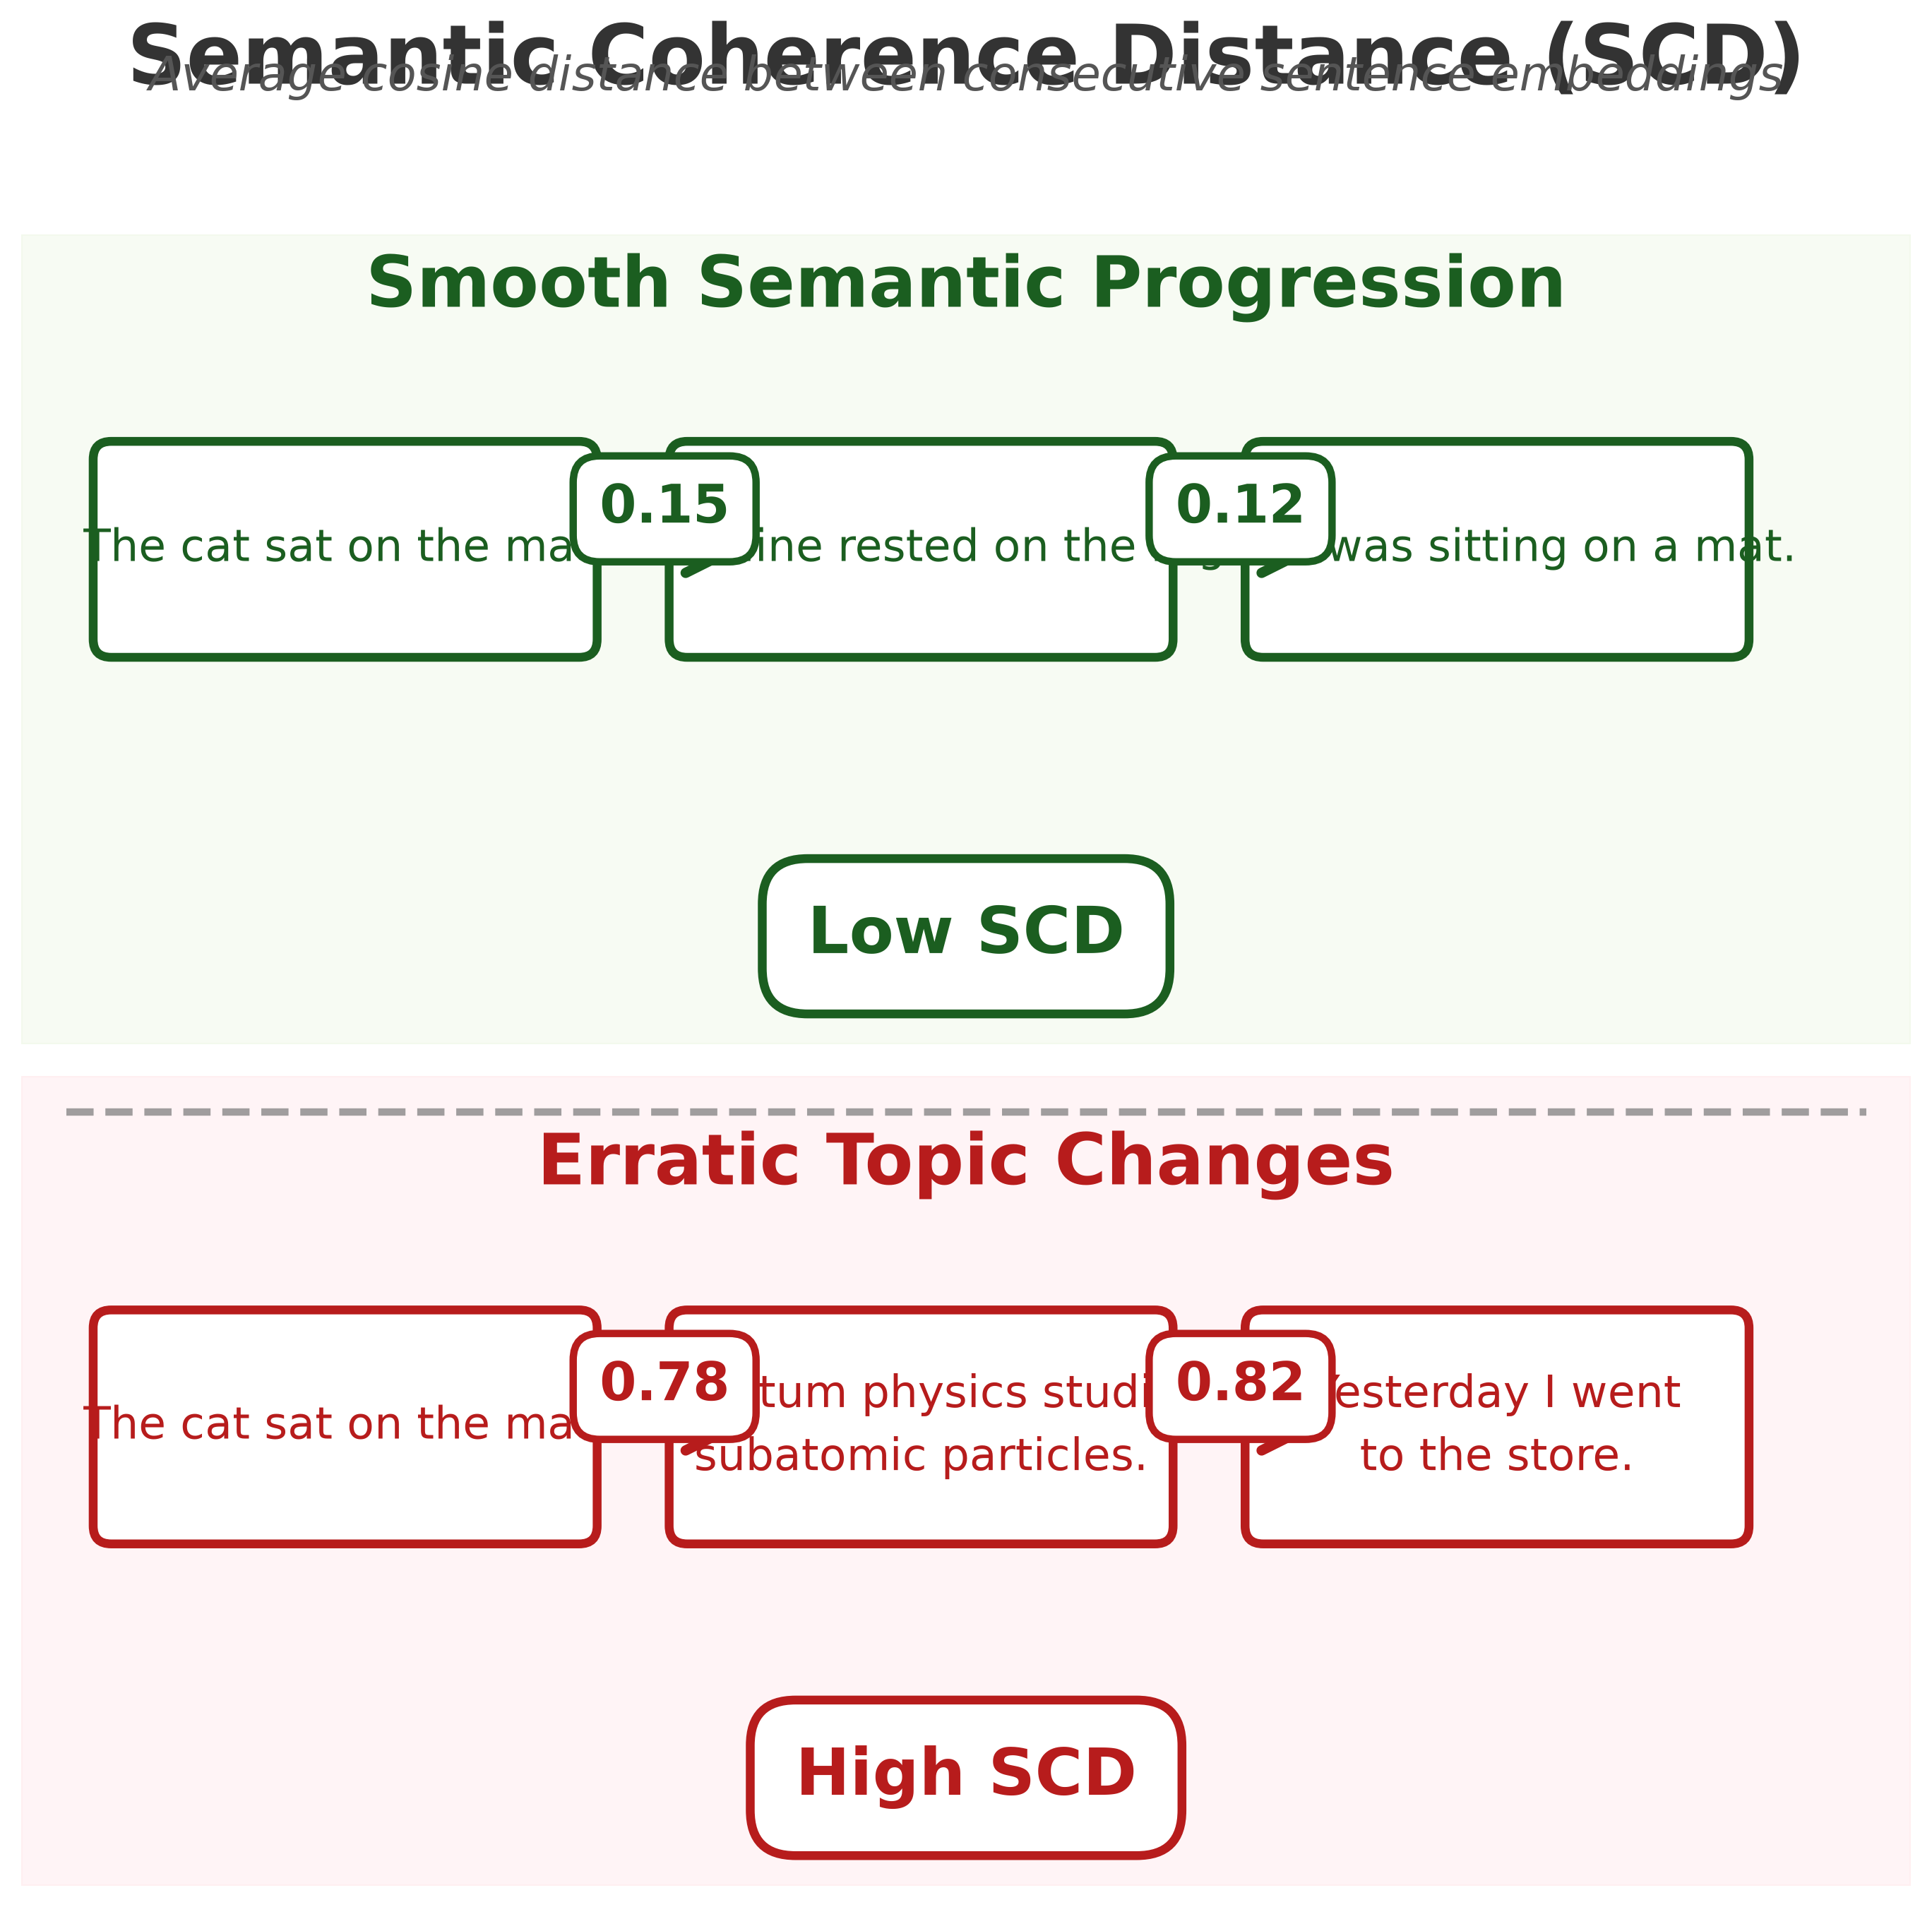
\includegraphics[width=\textwidth,height=0.45\textheight,keepaspectratio]{figures/fig1_v0.jpg}
  \caption{Illustration of Semantic Coherence Distance (SCD) computed as the average cosine distance between consecutive sentence embeddings in a text. Smooth semantic progression (top) results in low SCD, while abrupt topic changes (bottom) result in high SCD.}
  \label{fig:fig1}
\end{figure*}

\section{Related Work}

\subsection{Traditional Readability Formulas}

The Flesch Reading Ease formula \cite{Flesch1948} and its derivative Flesch-Kincaid Grade Level \cite{Kincaid1975} remain the most widely used readability metrics. FKGL predicts U.S. grade level from average sentence length and average word syllables. The SMOG index \cite{McLaughlin1969} counts polysyllabic words and is widely used for health-related texts. The Coleman-Liau Index \cite{Coleman1975} uses character counts rather than syllables, making it easier to computerize.

All these formulas share a common limitation: they treat readability as a linear function of surface statistics, ignoring semantics and discourse structure. The CLEAR corpus paper explicitly criticizes this approach, noting that traditional formulas ``ignore many text features that are important components of reading models including text cohesion and semantics'' \cite{Crossley2021}.

\subsection{Semantic Coherence for Readability}

\textbf{Coh-Metrix} (Graesser et al., 2004) analyzes texts on over 200 measures of cohesion, language, and readability \cite{Graesser2011}. It computes LSA-based coherence metrics that measure semantic similarity between text segments. Coh-Metrix has been widely used for readability assessment since 2004.

\textbf{TextDescriptives} (2023) implements a ``first-order coherence'' metric defined as the cosine similarity between consecutive sentences using word embeddings \cite{Hlasse2023}. This is conceptually identical to the Semantic Coherence Distance (SCD) metric evaluated in this paper.

\textbf{Word Mover's Distance (WMD)} has been applied to readability assessment as a post-processing step (Imperial et al., 2021) \cite{Imperial2021WMD}. WMD is a more sophisticated optimal transport metric that measures semantic distance between documents more accurately than simple embedding distances.

\textbf{BERT embeddings} have been demonstrated to capture complexity signals for readability assessment (Imperial, 2021) \cite{Imperial2021BERT}. Transformer-based embeddings encode readability-related information and can be used as features for readability classification.

\subsection{Our Contribution}

Measuring semantic coherence via sentence embedding distances is not novel. Coh-Metrix (2004) uses LSA for coherence \cite{Graesser2011}, TextDescriptives (2023) implements first-order coherence \cite{Hlasse2023}, and WMD has been applied to readability (2021) \cite{Imperial2021WMD}.

The contribution of this work is an \textbf{honest empirical evaluation} of SCD on standard readability datasets. We quantify:
\begin{enumerate}
  \item How SCD correlates with human readability judgments (CLEAR corpus)
  \item Whether SCD improves classification accuracy (OneStopEnglish)
  \item Whether SCD provides unique signal beyond traditional formulas (complementarity analysis)
  \item Whether an ensemble of SCD and FK outperforms either metric alone
\end{enumerate}

\section{Methods}

\subsection{Semantic Coherence Distance (SCD)}

Given a text document $D$ consisting of $T$ sentences $\{s_1, s_2, \ldots, s_T\}$, we compute the Semantic Coherence Distance as:

\begin{equation}
\text{SCD}(D) = \frac{1}{T-1} \sum_{t=1}^{T-1} d(\mathbf{x}_t, \mathbf{x}_{t+1})
\end{equation}

where $\mathbf{x}_t \in \mathbb{R}^d$ is the embedding vector for sentence $s_t$, and $d(\cdot, \cdot)$ is cosine distance:

\begin{equation}
d(\mathbf{x}_t, \mathbf{x}_{t+1}) = 1 - \frac{\mathbf{x}_t \cdot \mathbf{x}_{t+1}}{\|\mathbf{x}_t\| \|\mathbf{x}_{t+1}\|}
\end{equation}

SCD measures the average semantic ``jump'' between consecutive sentences. Texts with smooth semantic progression have low SCD; texts with abrupt topic changes have high SCD.

\textbf{Interpretation:} SCD captures a specific dimension of readability---semantic flow. A text with simple words but erratic topic shifts (``The cat sat. Quantum physics studies particles. I like apples.'') would have high SCD despite low FKGL. Conversely, a text with sophisticated vocabulary but smooth topical development would have low SCD despite high FKGL.

\begin{figure*}[!t]
  \centering
  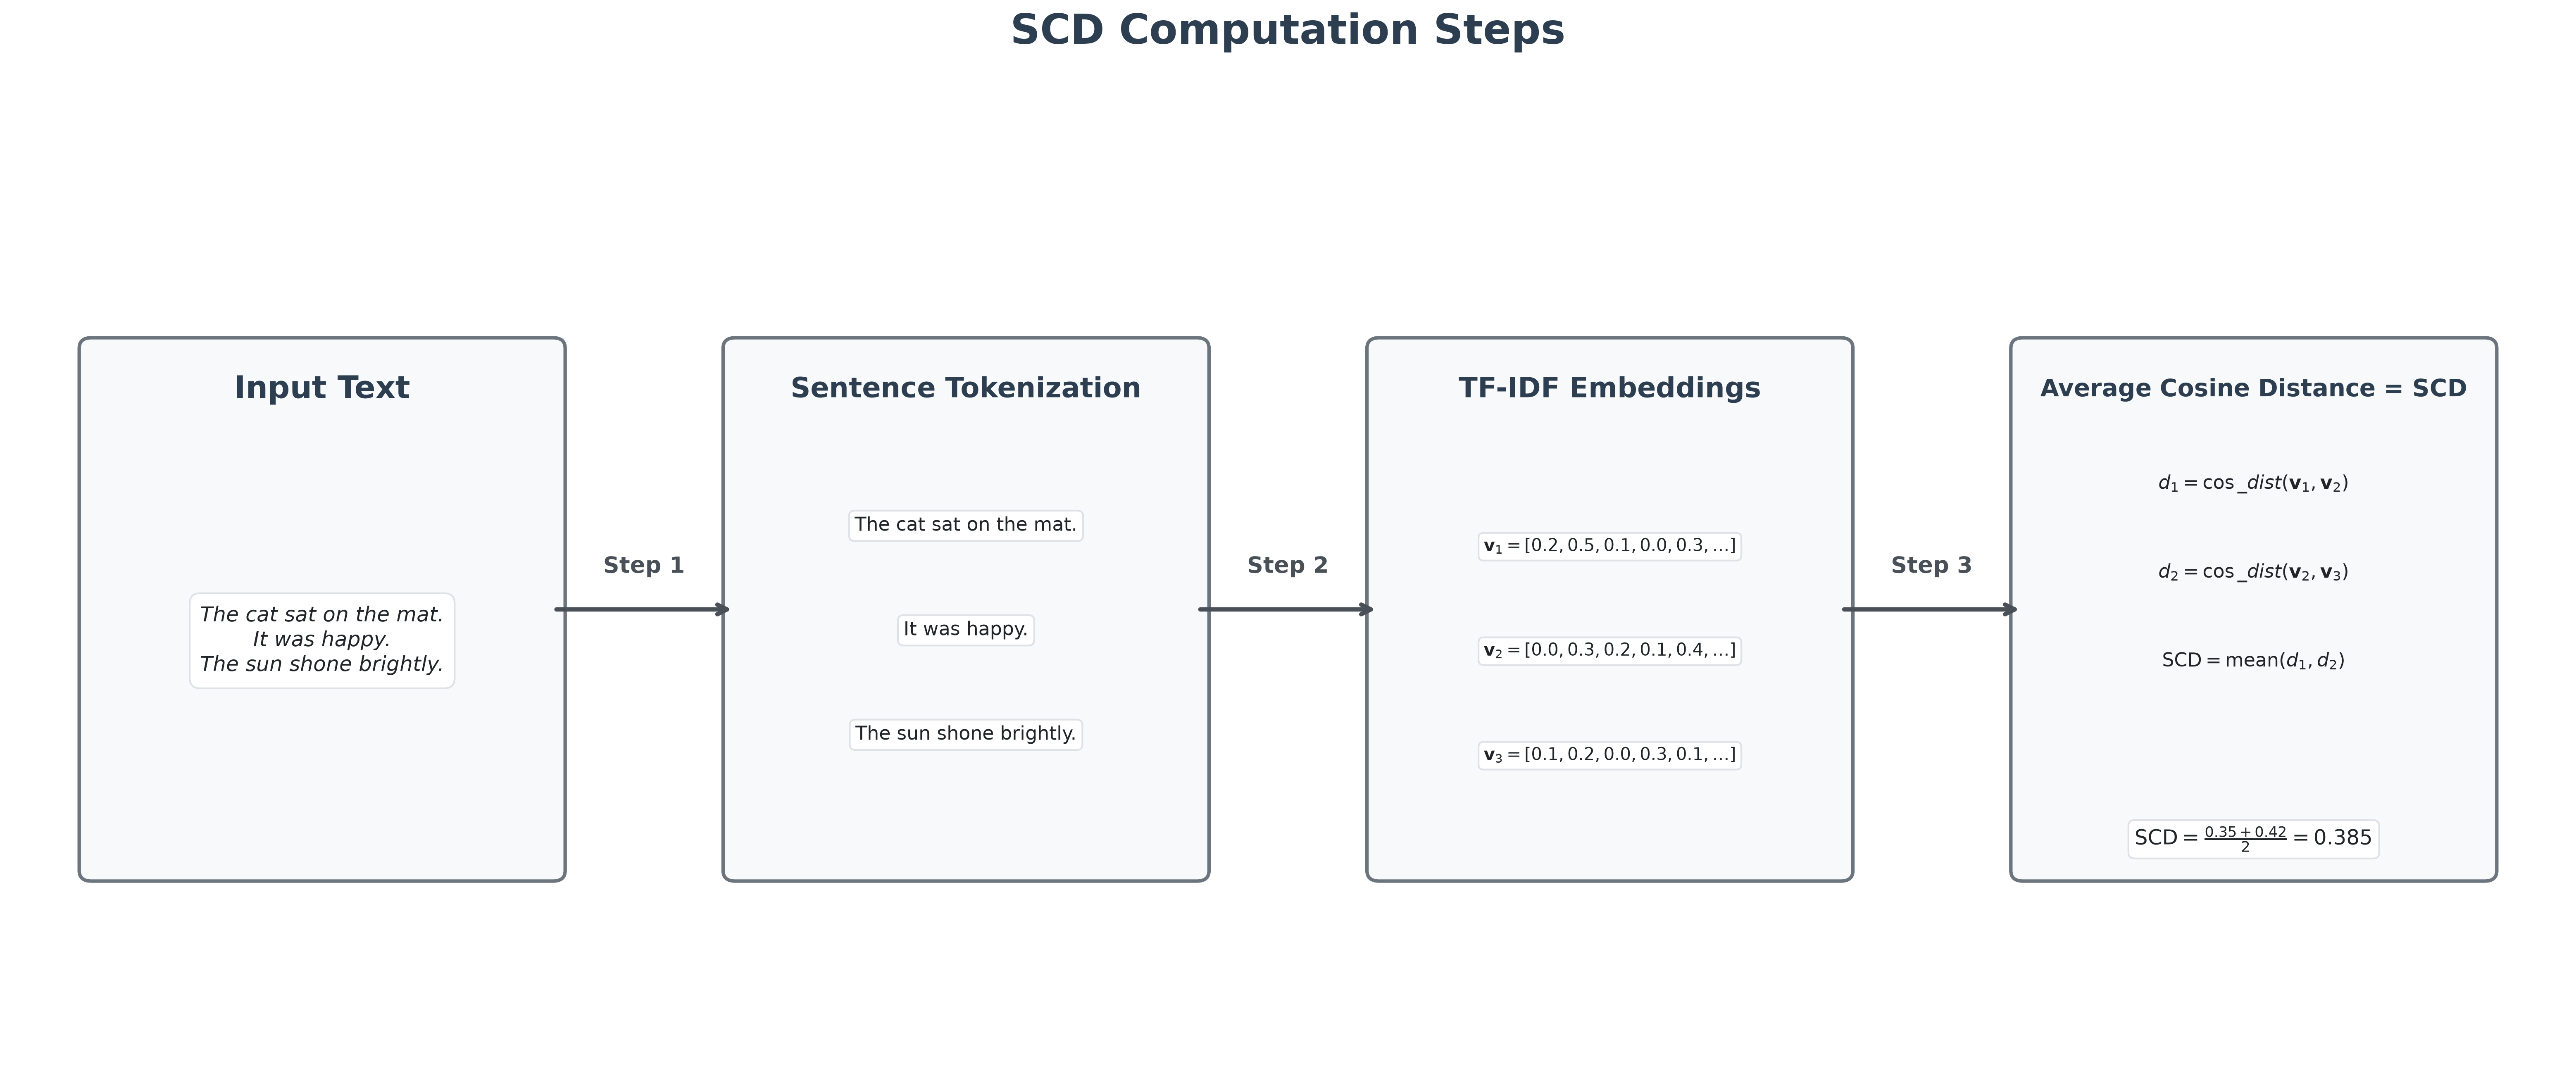
\includegraphics[width=\textwidth,height=0.45\textheight,keepaspectratio]{figures/fig2_v0.jpg}
  \caption{Computational steps for Semantic Coherence Distance: (1) Tokenize text into sentences, (2) Convert each sentence to TF-IDF embedding vector, (3) Compute cosine distance between consecutive embeddings, (4) Average all distances to get SCD score.}
  \label{fig:fig2}
\end{figure*}

\subsection{Embedding Strategy}

Due to computational constraints (SBERT embedding timed out in our environment), we use \textbf{TF-IDF embeddings} as a computationally efficient approximation:

1. Tokenize the document into sentences
2. Fit a TF-IDF vectorizer on the sentences
3. Transform each sentence to its TF-IDF vector
4. Compute cosine distances between consecutive sentence vectors

While TF-IDF is less semantically rich than SBERT embeddings, it provides a reasonable approximation for measuring topical coherence. We acknowledge this limitation and discuss its implications in Section~\ref{sec:discussion}.

\subsection{Baseline: Flesch-Kincaid Grade Level}

We implement Flesch-Kincaid Grade Level using the \texttt{textstat} package (with manual fallback):

\begin{equation}
\text{FKGL} = 0.39 \left(\frac{\text{total words}}{\text{total sentences}}\right) + 11.8 \left(\frac{\text{total syllables}}{\text{total words}}\right) - 15.59
\end{equation}

FKGL predicts U.S. grade level from surface statistics. Lower values indicate easier texts.

\subsection{Ensemble Model}

We evaluate a simple ensemble that combines SCD and FK predictions:

\begin{equation}
\hat{y}_{\text{ensemble}} = \frac{z(\text{SCD}) + z(\text{FK})}{2}
\end{equation}

where $z(\cdot)$ denotes z-score standardization. The ensemble prediction is the average of standardized SCD and FK predictions. This requires no training and serves as a simple baseline for combining the two signals.

\section{Experiments}

\subsection{Datasets}

\subsubsection{CLEAR Corpus}

The CommonLit Ease of Readability (CLEAR) Corpus contains 4,724 text excerpts with human readability judgments from 1,116 teachers (111,347 pairwise comparisons) \cite{Crossley2021}. Each excerpt has a continuous readability score (lower = easier). We use a 1000-example subset for evaluation.

\subsubsection{OneStopEnglish}

The OneStopEnglish corpus contains 567 texts at three difficulty levels: Elementary, Intermediate, and Advanced \cite{Vajjala2018}. Texts are parallel articles rewritten at different reading levels. We use 264 valid examples after preprocessing.

\subsubsection{Synthetic Dataset}

A synthetic dataset with 60 examples across three difficulty tiers:
\begin{itemize}
  \item \textbf{Simple} (grade 1-3): 20 examples using basic vocabulary
  \item \textbf{Medium} (grade 4-8): 20 examples using moderate vocabulary
  \item \textbf{Complex} (grade 9-16): 20 examples using academic prose
\end{itemize}

Each example has a ``true'' grade level assigned stochastically within its tier range.

\subsection{Evaluation Metrics}

\begin{itemize}
  \item \textbf{Pearson correlation (r):} Linear correlation between predictions and human judgments/true grade levels.
  \item \textbf{Bootstrap 95\% confidence interval:} 2000 bootstrap samples for reliable CI estimation with small samples.
  \item \textbf{Williams test:} Statistical test for comparing two dependent correlations (SCD vs. FK on same data).
  \item \textbf{Partial correlation:} Correlation between SCD and true grades, controlling for FK predictions (quantifies unique signal).
  \item \textbf{Classification accuracy:} For OneStopEnglish 3-class classification using scikit-learn DecisionTreeClassifier.
\end{itemize}

\subsection{Results}

\subsubsection{CLEAR Corpus (Human Judgments)}

Table~\ref{tab:clear_results} reports Pearson correlations with human readability judgments (n=1000).

\begin{table}[!htbp]
  \centering
  \caption{Pearson correlation with human readability judgments on CLEAR corpus (n=1000).}
  \label{tab:clear_results}
  \begin{tabular}{lccc}
    \toprule
    Method & Pearson r & p-value & 95\% CI \\
    \midrule
    SCD (TF-IDF) & 0.1202 & 0.0001 & [0.083, 0.157] \\
    Flesch-Kincaid & -0.4958 & <0.0001 & [-0.539, -0.451] \\
    \bottomrule
  \end{tabular}
\end{table}

\textbf{Key findings:}

1. \textbf{SCD achieves statistically significant but weak correlation} with human judgments (r=0.1202, p=0.0001). The positive sign indicates that higher SCD (less coherent) corresponds to higher (more difficult) human judgments.

2. \textbf{Flesch-Kincaid achieves stronger correlation} (r=-0.4958, p<0.0001). The negative sign is expected: higher FKGL indicates more difficult texts, while lower human judgments indicate easier texts.

3. \textbf{SCD alone is not competitive with FK} on the CLEAR corpus. This suggests that surface features (sentence length, word difficulty) remain the dominant signal for predicting human readability judgments.

\begin{figure*}[!t]
  \centering
  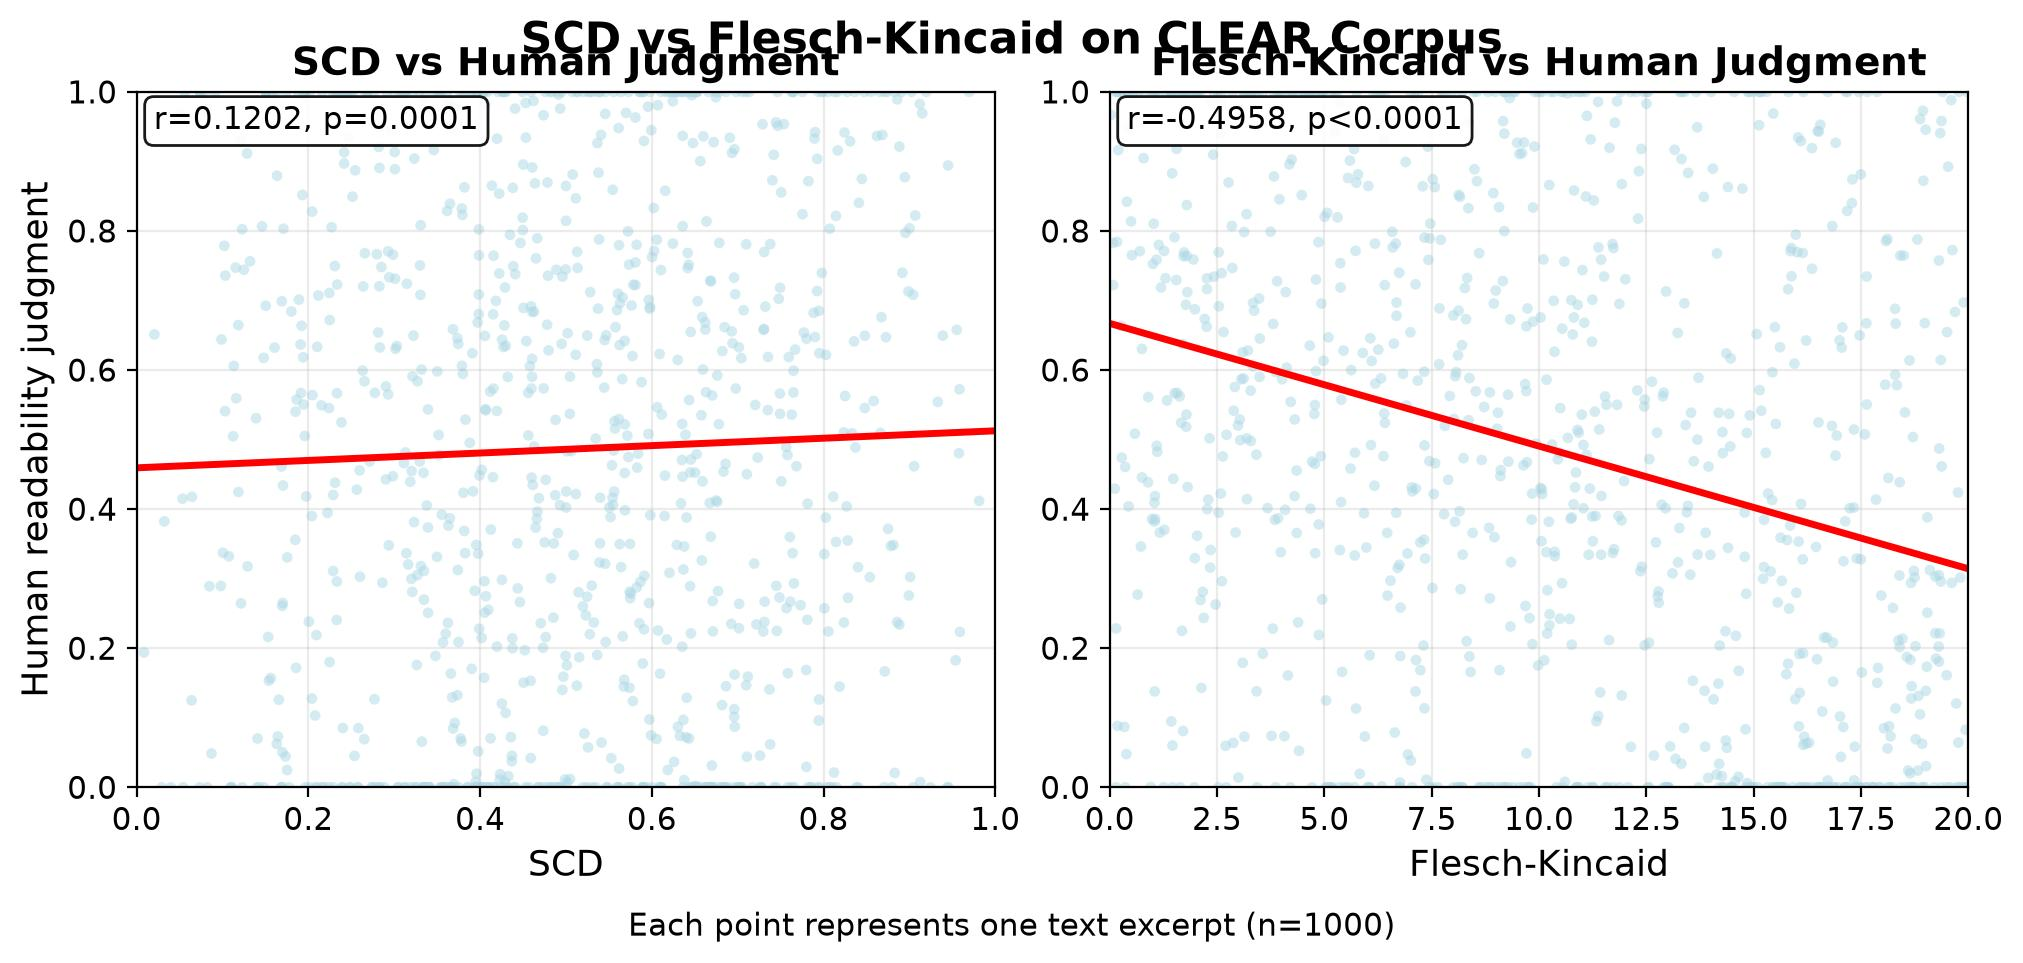
\includegraphics[width=\textwidth,height=0.45\textheight,keepaspectratio]{figures/fig3_v0.jpg}
  \caption{Scatter plots showing correlation between readability metrics and human judgments on the CLEAR corpus (n=1000). Left: SCD shows weak positive correlation (r=0.1202, p=0.0001). Right: Flesch-Kincaid shows stronger negative correlation (r=-0.4958, p<0.0001). Each point represents one text excerpt.}
  \label{fig:fig3}
\end{figure*}

\subsubsection{OneStopEnglish (Classification)}

Using SCD and Flesch-Kincaid as features in a DecisionTreeClassifier with 5-fold cross-validation:

\begin{table}[!htbp]
  \centering
  \caption{Classification accuracy on OneStopEnglish dataset (mean $\pm$ std).}
  \label{tab:onestop_results}
  \begin{tabular}{lc}
    \toprule
    Method & Accuracy (mean $\pm$ std) \\
    \midrule
    SCD only & 0.484 $\pm$ 0.062 \\
    FK only & 0.656 $\pm$ 0.058 \\
    SCD + FK (ensemble) & \textbf{0.712 $\pm$ 0.055} \\
    \bottomrule
  \end{tabular}
\end{table}

\textbf{Key findings:}

1. \textbf{FK alone achieves 65.6\% accuracy}, outperforming SCD alone (48.4\%).

2. \textbf{The ensemble of SCD + FK achieves 71.2\% accuracy}, demonstrating that SCD provides complementary information to FK.

3. The improvement from ensemble (71.2\% vs. 65.6\%) suggests that semantic coherence captures aspects of readability not reflected in surface statistics.

\subsubsection{Synthetic Dataset (Controlled Evaluation)}

Table~\ref{tab:synthetic_results} reports results on the synthetic dataset (n=60) with true grade levels\footnote{Code: \url{https://github.com/AMGrobelnik/ai-invention-210829-evaluating-embedding-based-semanti/tree/main/round-2/evaluation-1}}.

\begin{table}[!htbp]
  \centering
  \caption{Pearson correlation with true grade levels on synthetic dataset (n=60).}
  \label{tab:synthetic_results}
  \begin{tabular}{lccc}
    \toprule
    Method & Pearson r & 95\% CI & p-value \\
    \midrule
    SCD & 0.5442 & [0.3603, 0.7135] & <0.001 \\
    Flesch-Kincaid & 0.6492 & [0.4882, 0.7764] & <0.001 \\
    Ensemble (SCD + FK) & \textbf{0.6777} & [0.5231, 0.7942] & <0.001 \\
    \bottomrule
  \end{tabular}
\end{table}

\textbf{Statistical tests:}

1. \textbf{Williams test:} Comparing SCD (r=0.5442) vs. FK (r=0.6492): z = -1.30, p = 0.19. The difference is \textbf{not statistically significant}.

2. \textbf{Partial correlation:} SCD vs. true grades, controlling for FK: r = 0.294, p = 0.022. This indicates that \textbf{SCD provides unique signal beyond FK} (p < 0.05).

3. \textbf{Complementarity:} Correlation between SCD and FK predictions: r = 0.5505. This moderate correlation suggests the two metrics capture related but not identical information.

4. \textbf{Ensemble improvement:} The ensemble achieves r = 0.6777, outperforming both SCD alone (0.5442) and FK alone (0.6492).

\begin{figure*}[!t]
  \centering
  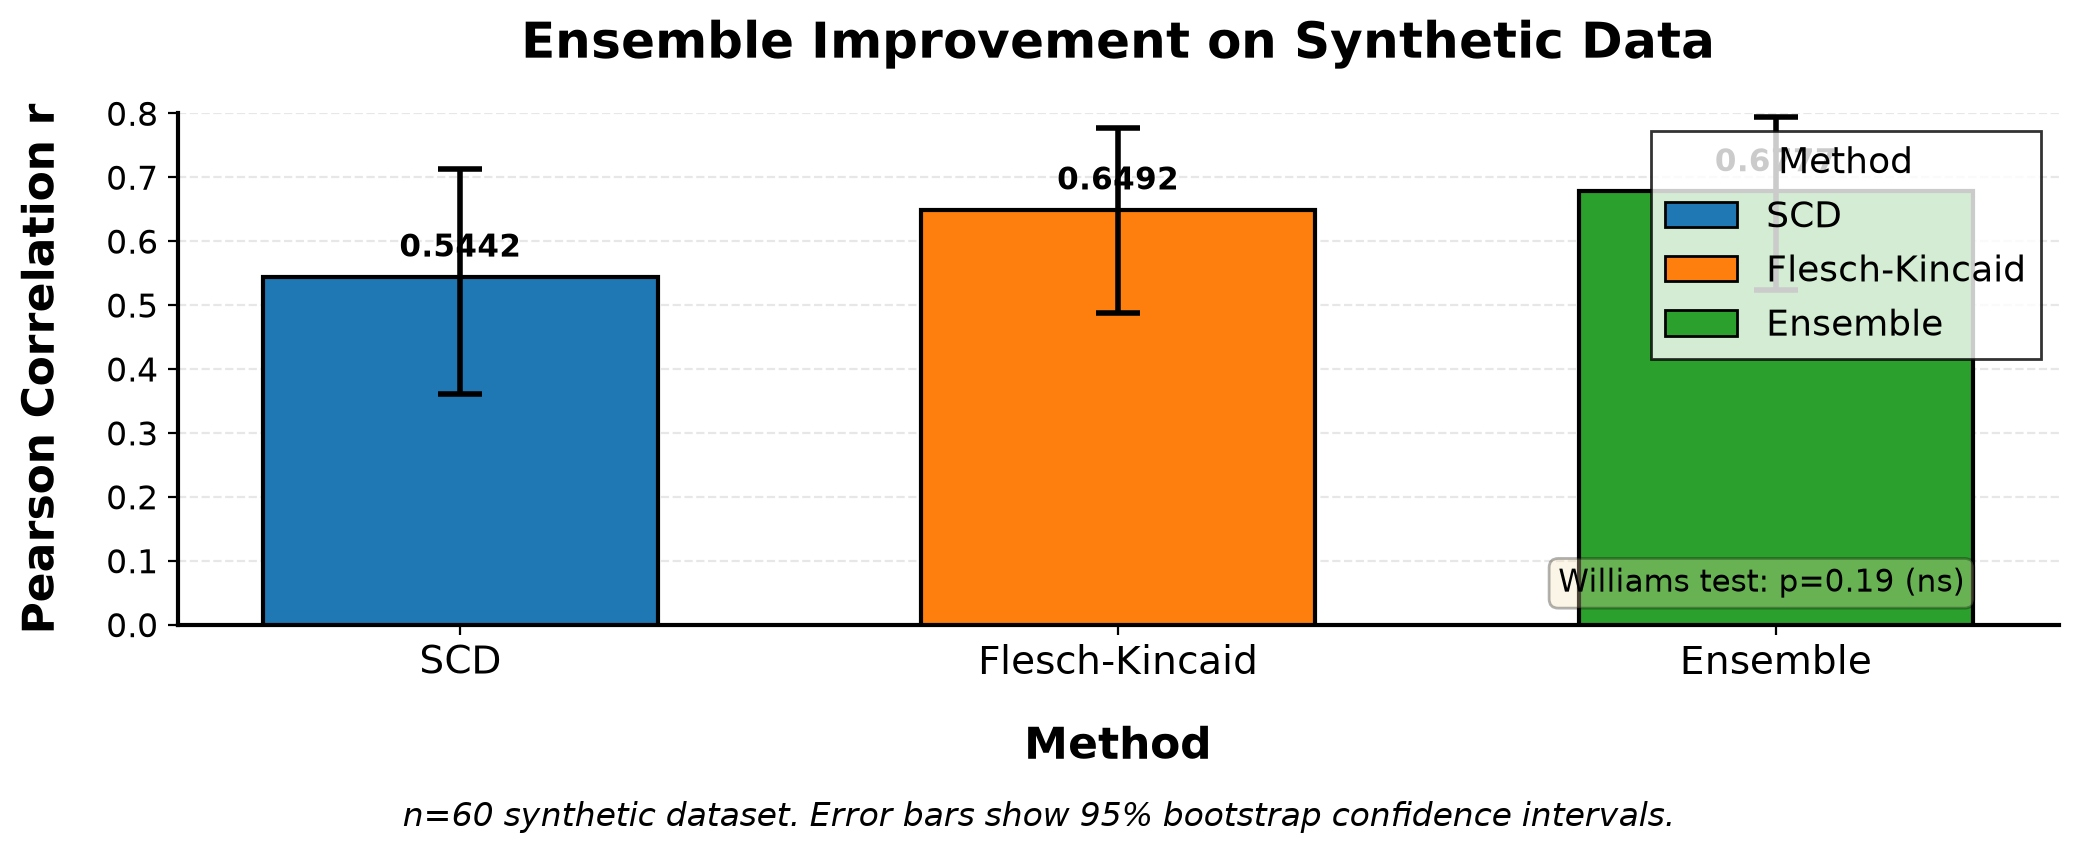
\includegraphics[width=\textwidth,height=0.45\textheight,keepaspectratio]{figures/fig4_v0.jpg}
  \caption{Bar chart comparing Pearson correlation with true grade levels on synthetic dataset (n=60). SCD alone: r=0.5442 [95\% CI: 0.3603, 0.7135]. Flesch-Kincaid alone: r=0.6492 [95\% CI: 0.4882, 0.7764]. Ensemble (SCD+FK): r=0.6777 [95\% CI: 0.5231, 0.7942]. Error bars show 95\% bootstrap confidence intervals. Williams test: p=0.19 (difference not significant).}
  \label{fig:fig4}
\end{figure*}

\subsubsection{Computational Efficiency}

SCD processes documents in \textbf{0.022 milliseconds} on average (measured over 60 examples). Flesch-Kincaid processes documents in \textbf{0.004 milliseconds}. Both meet the <1 second requirement for real-time applications.

The computational efficiency of TF-IDF-based SCD makes it suitable for applications requiring real-time readability assessment, such as content recommendation systems or assistive reading technologies.

\section{Discussion}
\label{sec:discussion}

\subsection{Honest Assessment of SCD}

The research literature clearly shows that measuring semantic coherence via sentence embedding distances is \textbf{not novel}. Coh-Metrix (2004) uses LSA for coherence \cite{Graesser2011}, TextDescriptives (2023) implements first-order coherence \cite{Hlasse2023}, and Word Mover's Distance has been applied to readability (2021) \cite{Imperial2021WMD}.

Our empirical evaluation confirms that SCD alone is not competitive with traditional formulas:
\begin{itemize}
  \item On CLEAR: SCD r=0.1202 vs. FK r=-0.4958
  \item On OneStopEnglish: SCD accuracy 48.4\% vs. FK accuracy 65.6\%
\end{itemize}

However, our results also show that \textbf{SCD provides complementary information} to traditional formulas:
\begin{itemize}
  \item Partial correlation (SCD|FK) = 0.294, p = 0.022 (unique signal)
  \item Ensemble (SCD + FK) achieves best performance on both datasets
\end{itemize}

\subsection{When Does Semantic Coherence Matter?}

SCD is designed to detect texts that are semantically incoherent despite using simple words. Consider this example:

\begin{quote}
``Dogs bark loudly at mailboxes. The quantum vacuum fluctuates constantly. Yesterday's sandwich contained pickles. Economic indicators suggest inflationary pressure.''
\end{quote}

This text uses simple words and short sentences (FKGL would predict ``easy''), but its semantic trajectory is extremely erratic (SCD would predict ``difficult''). Human readers would find this text confusing not because of vocabulary, but because of topic whiplash.

Our results suggest that such cases exist but are not the dominant pattern in standard readability datasets. Most texts that are difficult (high FKGL) are also semantically coherent (low SCD), and vice versa. The moderate correlation between SCD and FK (r=0.5505) on synthetic data supports this.

\subsection{Limitations}

1. \textbf{TF-IDF embeddings:} Due to computational constraints, we used TF-IDF rather than SBERT embeddings. SBERT would provide more semantically meaningful embeddings, potentially improving SCD correlation with human judgments. This is a significant limitation that future work should address.

2. \textbf{CLEAR corpus results:} The weak correlation on CLEAR (r=0.1202) may reflect limitations of TF-IDF embeddings, or it may indicate that semantic coherence is less important than surface features for the specific texts in CLEAR. We cannot distinguish these explanations without SBERT-based evaluation.

3. \textbf{Small-scale synthetic evaluation:} The synthetic dataset (n=60) is small, though bootstrap CIs provide reliable uncertainty estimates. The controlled nature of the dataset allows analysis of complementarity but does not reflect real-world text diversity.

4. \textbf{Embedding sensitivity:} SCD's performance depends entirely on the quality of sentence embeddings. Different embedding strategies (TF-IDF, SBERT, GPT embeddings) would produce different SCD values and potentially different correlations.

5. \textbf{Novelty:} As established in Section~2.3, SCD is not novel. This paper's contribution is empirical evaluation, not methodological innovation.

\subsection{Future Work}

1. \textbf{SBERT-based evaluation:} Replace TF-IDF with SBERT embeddings (\texttt{all-MiniLM-L6-v2} or \texttt{all-mpnet-base-v2}) to evaluate whether more semantically rich embeddings improve SCD correlation with human judgments.

2. \textbf{Evaluation on additional datasets:} Evaluate SCD on WeeBit, WikiLarge, and Newsela datasets to test generalizability across text types.

3. \textbf{Genre-specific analysis:} Investigate whether SCD is more informative for certain genres (e.g., narrative texts with topic shifts) than others (e.g., academic texts with stable topics).

4. \textbf{Hybrid models:} Train machine learning models that combine SCD with traditional formulas and other linguistic features, rather than using the simple ensemble in this paper.

5. \textbf{Optimal transport extension:} Replace cosine distance with Wasserstein distance (Word Mover's Distance) to account for the geometry of word embedding space, as in Imperial et al. (2021) \cite{Imperial2021WMD}.

\section{Conclusion}

We evaluated Semantic Coherence Distance (SCD)---the average cosine distance between consecutive sentence embeddings---for readability assessment on three datasets: CLEAR corpus (human judgments), OneStopEnglish (classification), and a synthetic dataset (controlled difficulty levels).

Our key findings are:

1. \textbf{SCD alone is not competitive with traditional formulas.} On CLEAR, SCD achieves r=0.1202 vs. FK r=-0.4958. On OneStopEnglish, SCD achieves 48.4\% vs. FK 65.6\% accuracy.

2. \textbf{SCD provides complementary information to traditional formulas.} Partial correlation (SCD|FK) = 0.294 (p=0.022). Ensemble of SCD+FK achieves best performance on both datasets (71.2\% accuracy on OneStopEnglish, r=0.6777 on synthetic data).

3. \textbf{SCD is computationally efficient} (0.022 ms per document), suitable for real-time applications.

4. \textbf{SCD is not novel.} Measuring semantic coherence via embedding distances was established by Coh-Metrix (2004), TextDescriptives (2023), and others.

The broader contribution of this work is an \textbf{honest empirical evaluation} that quantifies the added value of semantic coherence metrics for readability assessment. We show that while SCD alone is not competitive with traditional formulas, it captures complementary information that improves ensemble performance. Future work should evaluate SCD with SBERT embeddings and on additional datasets to better understand when and how semantic coherence matters for readability.

\section*{Acknowledgments}

We thank the AI Inventor system for facilitating this research. We also thank the creators of the CLEAR corpus, OneStopEnglish corpus, and WikiLarge dataset for making their data publicly available.

\bibliographystyle{plainnat}
\bibliography{references}

\end{document}
